\documentclass[english,paper=a4,DIV=calc]{scrartcl}
\usepackage{lmodern}
\usepackage[T1]{fontenc}
\usepackage[utf8]{inputenc}
\usepackage{babel}
\usepackage[numbers,sort&compress]{natbib}
\usepackage{graphicx}
\usepackage{siunitx}
\usepackage{todonotes}
\usepackage{enumitem}
\usepackage[autostyle=true,threshold=5,thresholdtype=words]{csquotes}
	\SetBlockEnvironment{quotation}
\usepackage{tikz}
	\usetikzlibrary{spy}
\usepackage{hyperref}

\makeatletter
\let\@fnsymbol\@arabic
\makeatother

\title{JAPPL-00642-2013\\Answer to reviewers}	
\author{%
	David Haberthür\footremember{psi}{Swiss Light Source, Paul Scherrer Institute, Villigen, Switzerland}
	\and Sébastien F. Barré\footremember{ana}{Institute of Anatomy, University of Bern, Switzerland}
	\and Stefan A. Tschanz\footrecall{ana}
	\and Eveline Yao\footrecall{ana}
	\and Marco Stampanoni\footrecall{psi}\ \superscript{, }\footremember{eth}{Institute for Biomedical Engineering, Swiss Federal Institute of Technology and University of Zürich, Switzerland}
	\and Johannes C. Schittny
		\footrecall{ana}\ \superscript{, }\footremember{contact}{Corresponding Author: Prof.\ Dr.\ Johannes C.\ Schittny, Institute of Anatomy, University of Bern, Baltzerstrasse 2, CH-3012 Bern, +41 31 631 46 35, \href{mailto:schittny@ana.unibe.ch}{schittny@ana.unibe.ch}}%
	}
\date{\today}

% Setup
\newcommand{\imsize}{\linewidth}
\newlength\imagewidth		% needed for scale bars
\newlength\imagescale		% ditto
\newcommand{\footremember}[2]{\footnote{#2}\newcounter{#1}\setcounter{#1}{\value{footnote}}}
\newcommand{\footrecall}[1]{\footnotemark[\value{#1}]}
\newcommand{\superscript}[1]{\ensuremath{^{\textrm{#1}}}}
\newcommand{\subscript}[1]{\ensuremath{_{\textrm{#1}}}}

\begin{document}
\maketitle

We thank both reviewers for their thorough work and appreciate their helpful advice. Below we answer their requests and explain our updates to the manuscript in detail.

\section{Replies for Reviewer \#1}
\subsection{Major comments}

\blockquote{The use of a synchrotron light source makes it impossible that this method will ever become routine. Looking at the imaging datasets I am wondering whether the whole study could not have been done \textelp{} by \textelp{} microCT?}

To fully extract multiple acini which are located close together in the tip of the right lower lung lobe we looked at, we needed to acquire tomographic datasets containing a large lung volume (up to \(4.5\times4.5\times\SI{4.5}{\cubic\milli\meter}\)).
To be able to segment the razor-thin septa between the alveoli, which are in the order of several \si{\micro\meter}, we needed to acquire tomographic datasets with very high resolution (in our case \SI{1.48}{\micro\meter} voxel side length).

As \citet{Vasilescu2013} have shown, reaching to both these goals is possible for small regions of interest with microCT imaging, but requires a rather cumbersome multi-step process; at first a low resolution, high volume overview scan, detection of the region of interest and then a high resolution, low volume scan of the desired region of interest (at exactly the desired, registered location).
At least in our \si{\micro}CT, the samples were too large for a high resolution scan.
We could have cut the sample, but it would have destroyed the region of interest.

To overcome these constraints, we employed a single-step method to provide both high resolution and high volume tomographic scans (as described in detail in our previous publication \citep{Haberthuer2010}.

With other methods available to us (Skyscan microCT available at the Institute of Anatomy, University of Bern), we would not have been able to reach our goal, since the resolution of the tomographic scans is not high enough to unambiguously segment the dataset down to the level of single alveoli, as shown in \autoref{fig:uct}.

\renewcommand{\imsize}{\linewidth}
% \\anatera7\MicroCT\R253C60L\rec_png8Bit\R253C60L__rec1928.PNG
\begin{figure}[htb]
	\centering
	\pgfmathsetlength{\imagewidth}{\imsize}%
	\pgfmathsetlength{\imagescale}{\imagewidth/3255}%
	\def\x{2012}% scalebar-x at golden ratio of x=3255px
	\def\y{1850}% scalebar-y at 90% of height of y=2055px
	\begin{tikzpicture}[x=\imagescale,y=-\imagescale,spy using outlines={red, circle, magnification=2.5, size=25 * 2.5, connect spies}]
		\clip (0,0) rectangle (3255,2055);
		\node[anchor=north west, inner sep=0pt, outer sep=0pt] at (0,0) {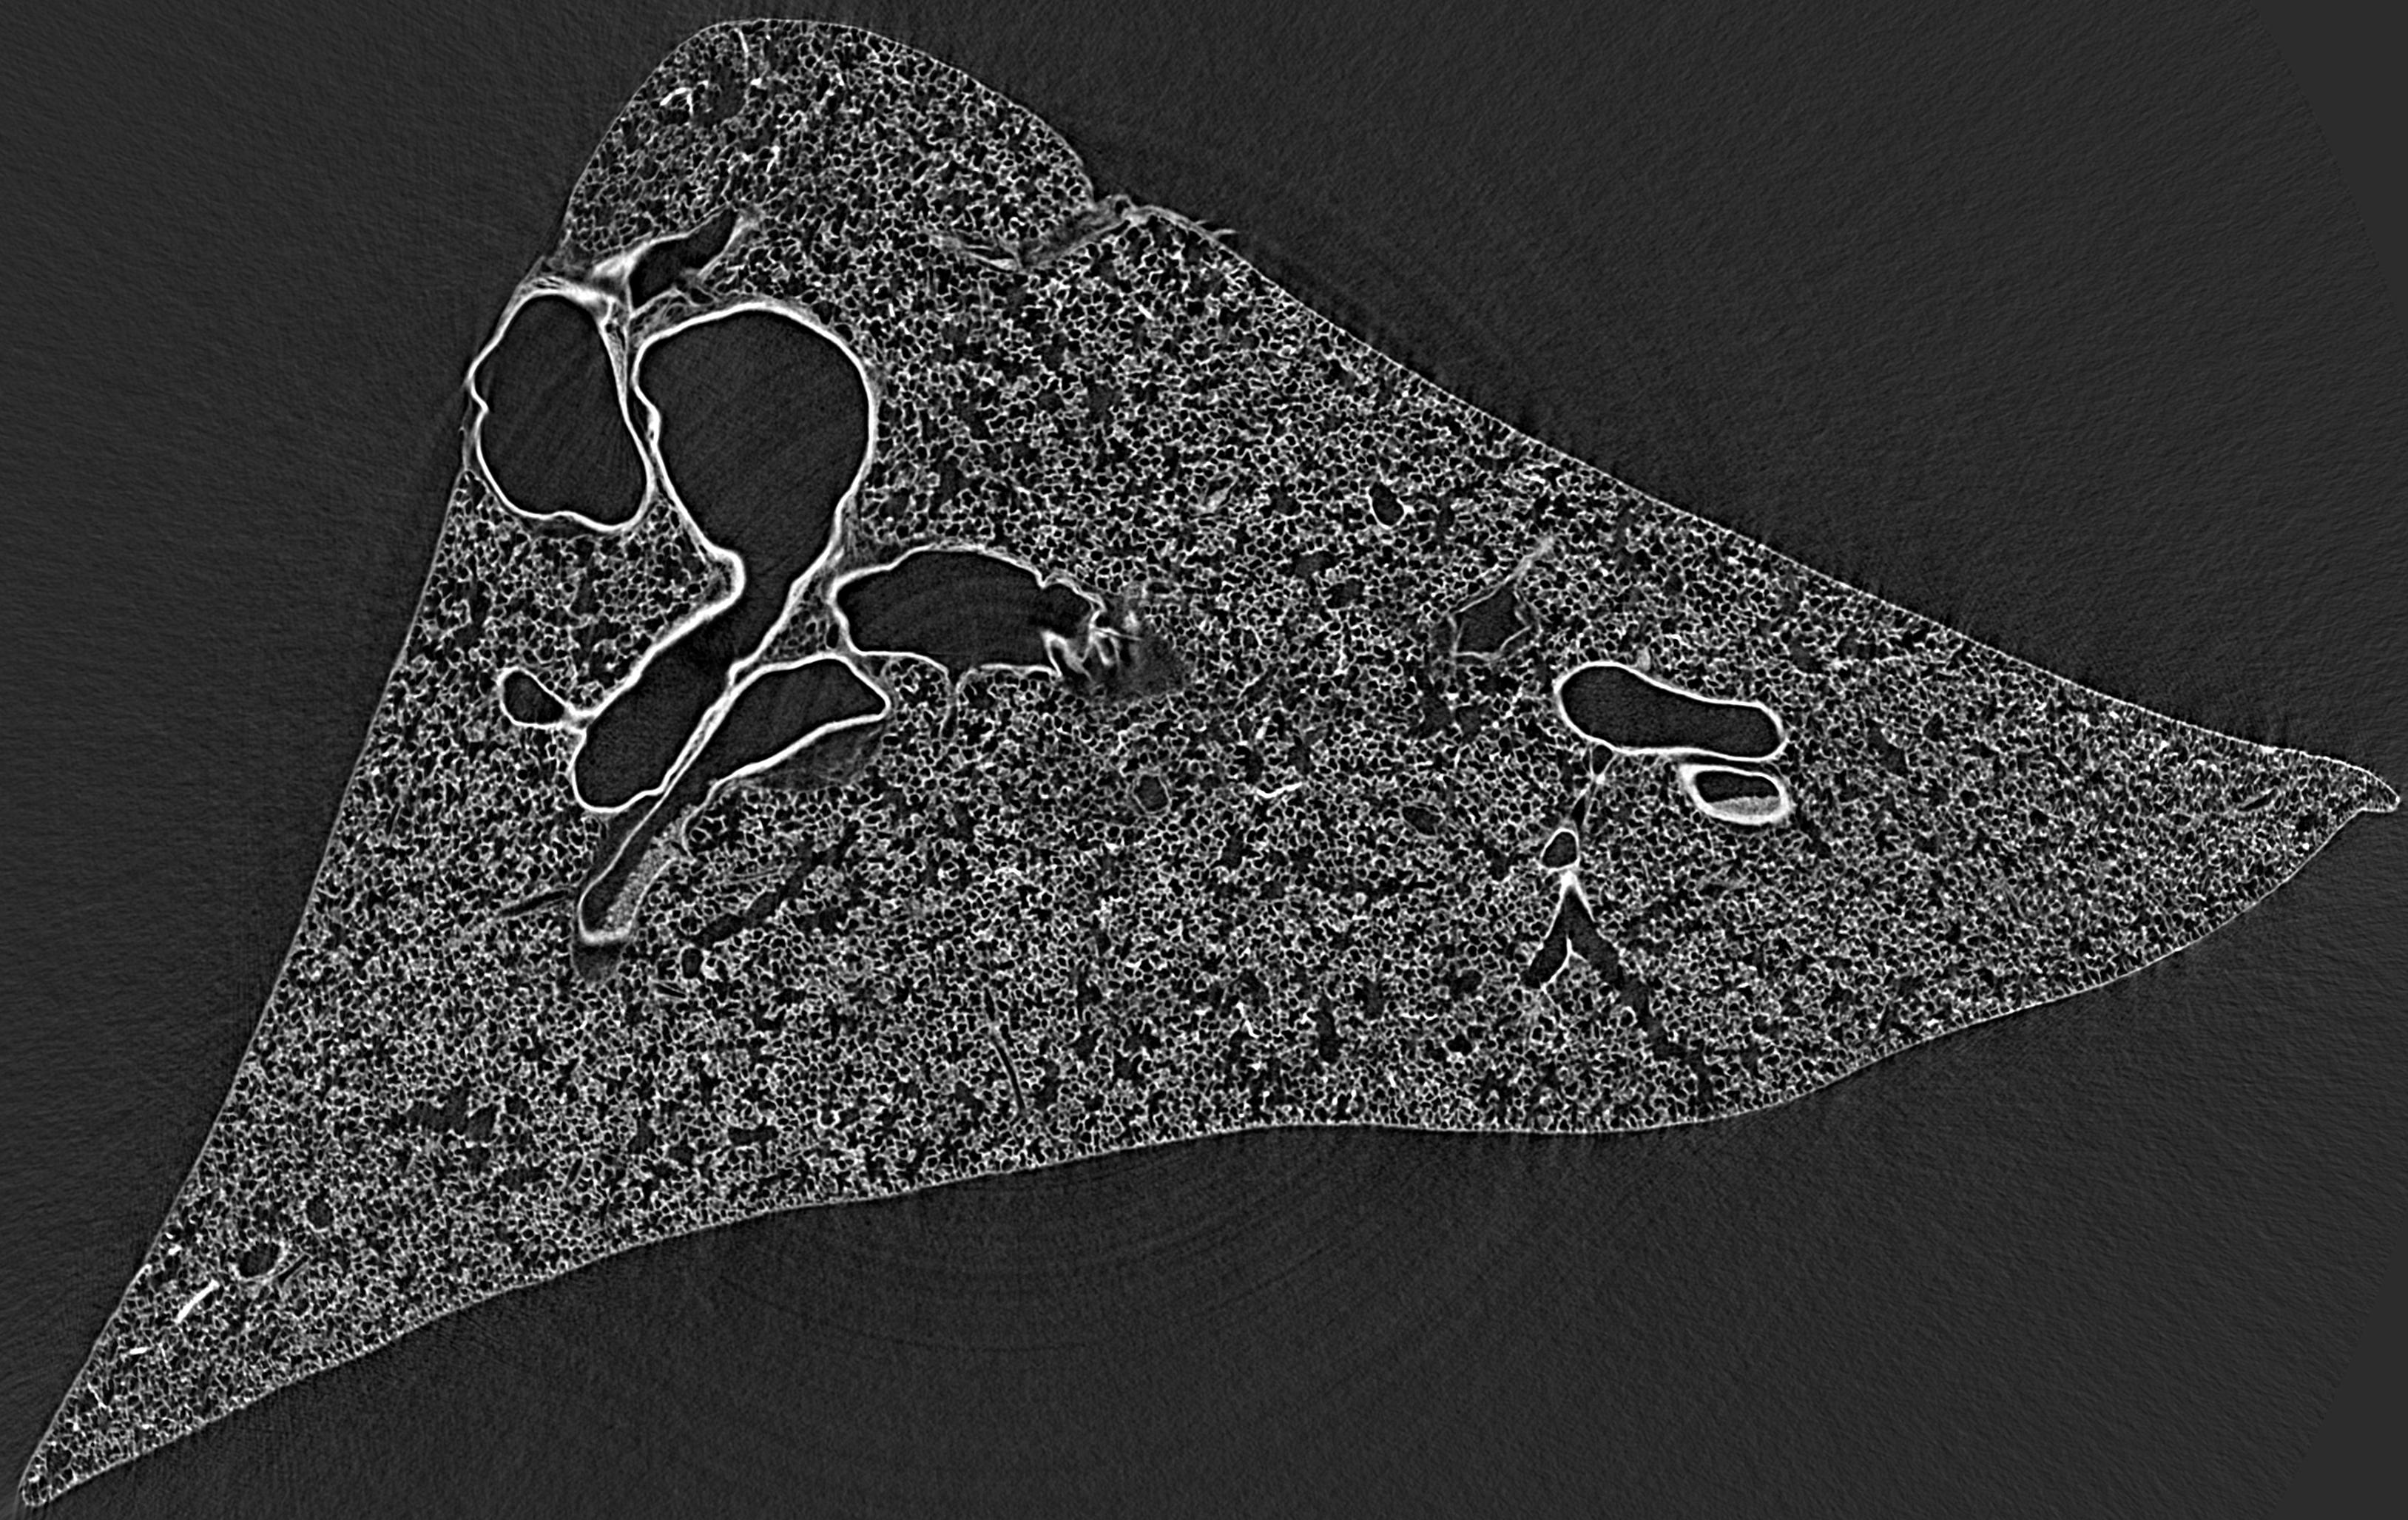
\includegraphics[width=\imagewidth]{img/R253C60L__rec1928_crop_enhance}};
		% 3255px = 10.5787mm > 100px = 325um > 154px = 500um, 31px = 100um
		\draw[|-|,white,thick] (\x,\y) -- (\x+154+154,\y) node [midway,above] {\SI{1}{\milli\meter}};
		\spy on (200,1860) in node at (1100, 1600);
		\spy on (1480,900) in node at (400, 400);
		\spy on (2100,900) in node at (2700, 400);
		\spy on (2300,1300) in node at (2800, 1600);
	\end{tikzpicture}%
	\caption{Slice of tomographic dataset obtained from criticl point dried rat lung sample (day 60, from another study) scanned with a Skyscan 1172 \si{\micro}CT by Sébastien Barré.
		The combination of voxel size of size \SI{3.25}{\micro\meter}, lower contrast and image artifacts hinder a proper segmentation.
		Zoomed insets (\(2.5\times\) magnification) show examples of such problems.}
	\label{fig:uct}
\end{figure}

Additionally, especially, since Reviewer \#2 specifically suggested to discuss two publications with results also obtained at synchrotron radiation facilities \citep{Sera2013,Xiao2013}, we still feel that our research has merit and several advantages, despite the limited availability of synchrotron radiation facilities.

\blockquote{Looking at the imaging datasets I am wondering whether the whole study could  not have been done with much less effort by using alternative (smaller, cheaper) imaging modalities, e.g. microCT? This point certainly deserves discussion.}
We tried to address this specific concern in the Materials and Method section of our manuscript and hope to have answered it there and above in sufficient detail.

\subsection{Minor comments}
We implemented all of the suggested changes and excuse ourselves for the typographic errors. Some of the suggestions merit a detailed explanation, which follows after the specific comments:

\begin{enumerate}[start=3]
	\item \textelp{} Why was paraffin (which is known to induce tissue shrinkage) used? Was shrinkage measured?
\end{enumerate}

We tested several embedding methods and finally settled on paraffin embedded samples for this study.
Details as well as disadvantages of each embedding method are specified in the list below.
Naturally we measured the tissue shrinkage and corrected for it in the stereological estimations, where applicable.
We added this information in the manuscript.

\begin{description}
	\item [Epon embedding] First studies were performed with Epon-embedded and heavy-metal stained rat lung samples, some even cylindrically shaped on a watchmakers lathe.
		Since Epon has a fairly large absorption coefficient, the signal-to-noise ratio of the resulting tomographic datasets did not permit a proper segmentation.
	\item [Critical point drying] Dried, heavy-metal stained rat lung samples were not stable enough to perform the tomographic experiments at the radiation level at TOMCAT, tomographic datasets showed non-negligible motion artefacts preventing successful reconstruction of the data.
	\item [Untreated samples] We also scanned unstained rat lung samples at TOCMAT and performed tomographic reconstructions with phase retrieval methods to increase the contrast in the low-absorbing tissue~\citep{Marone2011}.
	Even though we were able to increase the contrast, phase retrieval methods and subsequent filtering generally involves a certain loss of resolution in the resulting tomographic datasets, which we needed to avoid.
	\item [Paraffin] Even though paraffin embedded samples suffer from tissue shrinkage, this shrinkage can be measured and the results can be corrected for this shrinkage.
	Scanning paraffin embedded heavy-metal stained samples provided the safest and easiest route to achieve reproducible and consistent results.
\end{description}

Paraffin embedding and heavy-metal staining was thus the preparation method that was best suited for us to achieve the desired results, high quality tomographic datasets for subsequent image processing and stereological analysis.

\begin{enumerate}[start=5]
	\item \textelp{} Although the statement that an estimation of morphometric parameters assigned to one particular acinus is not possible by LM is correct, a LM-based stereological method for estimation of the number of ventilatory units \textelp{} exists: Authors should consult (and discuss) a paper by \citet{Wulfsohn2010}.
\end{enumerate}
We never intended to claim that there is no method to estimate the total number of ventilatory units/acini in a lung from LM images and clarified this paragraph thanks to this suggestion.

\section{Replies for Reviewer \#2}
\subsection{Major comments}
\blockquote{Although studies with high-resolution lung imaging are not that common, the authors are missing some recent and relevant articles about acinar level imaging in small animals: \textins{specifically mentioning publications \citep{Xiao2013,Sera2013,Kumar2013}} \textelp{}}

We thank reviewer \#2 for suggesting these studies and added a discussion of the relevant results to the manuscript.

\subsection{Minor comments}
Additionally to some minor clarifications in the text, this reviewer also suggests that we equally scale the plots in Figure 6, since. 

\blockquote{it would be easier to compare the images if they were scaled in the same scale.}

As far as we see it, the y-scale (acinar volume) of the plots is equal for all six subplots.
The x-position of the acini only specifies their bijective index number.
We feel that equally scaling the x-axis range (index number of acinus) for all six plots would not add any information, since we have a different amount of extracted acini for each animal (24, 10 and 9).
We thus did not change the scaling.

Maybe we misunderstood this specific comment, in this case we kindly ask the second reviewer to clarify it and we are willing to change the figure accordingly.

\bibliographystyle{unsrtnat}
\bibliography{../../library}
%\bibliography{/afs/psi.ch/user/h/haberthuer/Documents/library}

\end{document}

